% This is samplepaper.tex, a sample chapter demonstrating the
% LLNCS macro package for Springer Computer Science proceedings;
% Version 2.20 of 2017/10/04
%
\documentclass[runningheads]{llncs}
%
\usepackage{graphicx}
\usepackage{enumitem}
\usepackage{url}
% Used for displaying a sample figure. If possible, figure files should
% be included in EPS format.
%
% If you use the hyperref package, please uncomment the following line
% to display URLs in blue roman font according to Springer's eBook style:
% \renewcommand\UrlFont{\color{blue}\rmfamily}

\begin{document}

\begin{titlepage}
    \centering
    
\includegraphics[width=0.8\textwidth]{image.jpeg}\par % Adjust the width as needed
     \vspace{2cm}
    {\scshape\large SOEN6841 : Topic Analysis and Synthesis Report \par}
    \vspace{1.5cm}
    {\scshape\Huge Establish control initially when my project is huge\par}
    \vspace{1.5cm}
    \vspace{1.5cm}
    {\large Advisor: Professor Pankaj Kamthan\par}
    \vspace{1.5cm}
    {\large By: Kevin Jivani (Student ID: 40226491)\par}
    \vspace{1cm}
    {\large \today\par}
\end{titlepage}

\setcounter{tocdepth}{3}
\setcounter{secnumdepth}{3}
\tableofcontents
\newpage


\section*{Abstract}
This report investigates strategies for establishing initial control in large-scale projects, addressing challenges posed by their complexity and scope. Focusing on strategic decomposition, project planning, and communication strategies, the research explores how these elements contribute to effective control mechanisms. Key findings highlight the pivotal role of decomposition in fostering collaboration, the significance of initiation and planning phases, and the impact of communication on employee performance. The report proposes an evaluation framework for software project initiation, offering a structured approach to assess and improve initiation processes. Overall, it provides actionable insights for project managers navigating the intricacies of managing extensive projects.
\newpage

\section{Introduction}


\subsection{Problem Statement}
Large scale projects pose unique set of challenges, demanding attention to initial control measures. As projects scale in complexity and scope, establishing effective control mechanisms at the outset becomes a critical concern. This report explores the topic of "How to establish control initially when my project is huge". The magnitude of tasks, resource allocation, and intricate interdependencies can overwhelm traditional project management approaches, necessitating a comprehensive understanding of the factors influencing initial control. This analysis seeks to explore the specific hurdles faced when dealing with vast projects, aiming to identify strategies, frameworks, and best practices that empower project managers to establish robust control mechanisms from the project's inception.


\subsection{Motivation}

In navigating the complexities of large-scale projects, the pivotal role of decomposition cannot be overstated. The initial stages demand a strategic breakdown of the project into manageable components, for clarity and control. Effective leadership is crucial in steering the initiation and planning phases, setting the tone for program control. The planning process becomes key, particularly in addressing dependencies, providing a structured framework for effective management. Communication strategies and robust infrastructure emerge as lifelines, essential for managing interactions and sustaining control in the dynamic landscape of large programs. This analysis aims to uncover the role of these elements in establishing control within expansive project landscapes.


\subsection{Research Question}
\begin{itemize}[label=$\bullet$]
    \item How to strategically decompose a large project ? 
    \item What are different way to plan a project ?
    \item How can effective communication help in large scale projects?
\end{itemize}

\subsection{Objective}

\begin{itemize}[label=$\bullet$]
    \item \textbf{Decomposition of Project:}
    Investigate how the strategic decomposition of large projects contributes to establishing effective control mechanisms in the initial stages.
    
    \item \textbf{Project Planning Methods:}
    Explore different methods of project planning for better control, with a focus on managing dependencies within the intricate landscape of large-scale endeavors.

    \item \textbf{Effective Communication Strategies :}
    Evaluate essential communication strategies for managing interactions and maintaining control in the dynamic environment of large programs.
\end{itemize}


\section{Methods and Methodology}


\subsection{Decomposing Big Projects}
Decomposition is pivotal in managing large-scale software projects, serving as a systematic approach to break down complex systems into manageable components. This process enhances development efficiency by fostering parallelism, enabling teams to work concurrently on distinct modules. Through decomposition, intricate tasks are subdivided into smaller, more comprehensible units, facilitating better coordination and collaboration among team members.


\subsubsection{Work Breakdown Structure}\mbox{}\\
A work breakdown structure (WBS) is a hierarchical decomposition of a project into smaller, more manageable components. It is a tool used by project managers to define and organize the project's scope of work, and to break it down into smaller, more manageable tasks. The WBS helps to ensure that all project work is accounted for, and that each task is assigned to the appropriate team member or organizational unit. It is an essential tool for effective project planning, execution, and control\cite{wbs}.

\begin{itemize}[label=$\bullet$]
    \item \textbf{Identify Project Phases: }
    Break down the software project into distinct phases or stages. Common phases might include requirements analysis, design, implementation, testing, and deployment. Each phase represents a major milestone in the project's life cycle.\\

    \item \textbf{Define Major Tasks within Each Phase:}
    For each identified phase, further decompose the work into major tasks or activities. For example, within the implementation phase, tasks may include coding, unit testing, and integration testing. Assign specific responsibilities to each task and define their dependencies.\\


    \item \textbf{Create SubTasks and Work Packages:}
    Break down major tasks into smaller, manageable sub-tasks or work packages. These should represent specific actions or deliverables that contribute to the completion of the major task. Ensure that each sub-task is well-defined, measurable, and has clear criteria for completion.\\

    \item \textbf{Assign Resources and Schedule:}
    Allocate resources (human, technological, and other necessary resources) to each work package. Create a timeline or schedule for the project by estimating the duration of each task and identifying dependencies between tasks. This helps in creating a realistic project timeline and managing resource allocation effectively.
        
\end{itemize}

\subsubsection{Component based project breakdown in PRINCE2}\mbox{}\\
In PRINCE2 (PRojects IN Controlled Environments)\ref{prince}, a project is broken down into several components using a structured approach. The key elements of project breakdown in PRINCE2 include:

\begin{itemize}[label=$\bullet$]
    \item \textbf{Project Management Team:}  
    PRINCE2 defines clear roles and responsibilities for individuals involved in the project. The project management team is typically composed of roles such as the Project Manager, Project Board, Team Manager, and Project Support. This establishes a hierarchy of accountability and ensures that each aspect of the project is overseen by the appropriate authority.\\

    \item \textbf{Processes:}
    PRINCE2 organizes project management into a set of processes, each representing a set of activities to be carried out during the project's lifecycle\cite{prince2}. These processes are:\\

        \begin{enumerate}
            \item \textbf{Starting up a Project (SU)}: Ensures that the project is viable and worthwhile.
            \item \textbf{Initiating a Project (IP)}: Defines the project's scope, objectives, and approach.
            \item \textbf{Directing a Project (DP)}: The high-level decision-making process involving the Project Board.
            \item \textbf{Controlling a Stage (CS)}: Manages each stage of the project and ensures that work is progressing according to plans.
            \item \textbf{Managing Product Delivery (MP)}: Ensures that work packages are developed and delivered effectively.
            \item \textbf{Managing a Stage Boundary (SB)}: Prepares for the next stage, ensuring that the Project Plan is updated.
            \item \textbf{Closing a Project (CP)}: Formalizes project closure, assesses its success, and learns lessons for future projects.\\
        \end{enumerate}

    \item  \textbf{Themes:}
    PRINCE2 incorporates seven themes that are applied throughout the project. These themes are integrated into the processes to ensure a holistic approach. The themes include Business Case, Organization, Quality, Plans, Risk, Change, Progress.\cite{prince3}
    
\end{itemize}




\subsection{Initiating and Planning Programs}

Software projects often face complexity, and a common shortcoming in the industry is the lack of comprehensive project initiation. The success of a software development project hinges significantly on the quality of its initiation. The planning and initiating phases act as foundational pillars, establishing the project's groundwork. Planning involves defining objectives, scope, and deliverables with precision, analyzing requirements, allocating resources, and creating a structured timeline. This meticulous planning aims to mitigate risks and guide the team through the intricacies of software development.


\subsubsection{Evaluation Framework for Software Project Initiation}\mbox{}\\
Evaluation framework was proposed in \cite{evaluate}. The framework is developed based on the relationships between the components of the system request. The evaluation firstly starts with each component and then the relationships
between these components are calculated. Following are the key ideas of the framework. Figure \ref{fig:evalframework} shows the diagram of evaluation framework.

\begin{itemize}[label=$\bullet$]
    \item Identify the key elements of the software project request, including the project sponsor, business needs, business values, business requirements, and objectives.
    \item Use the quality criteria to evaluate each element and its relationships with other elements.
    \item Collect and analyze data to assess the effectiveness of the software project initiation and inform decision-making and improvement.
\end{itemize}

\begin{figure}
    \centering
    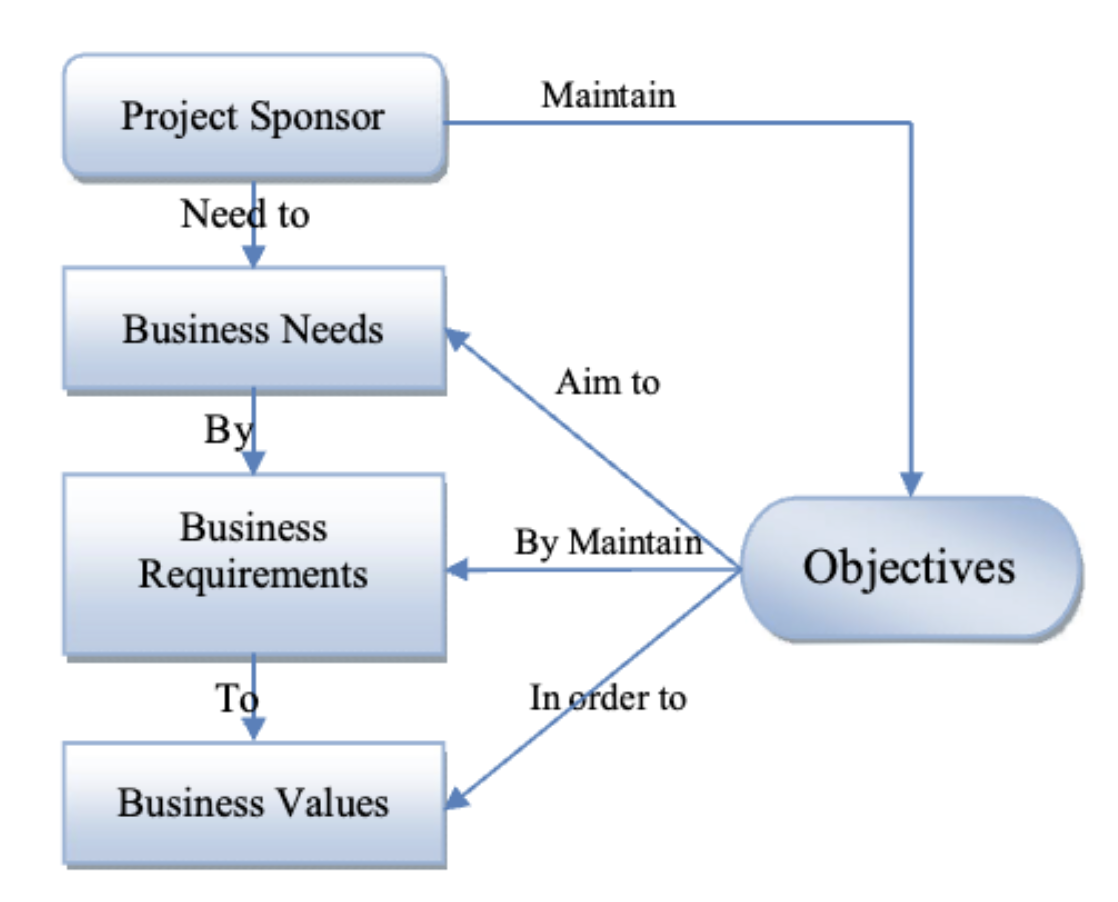
\includegraphics[width=0.8\linewidth]{EvaluationFramework.png}
    \caption{Evaluation Framework}
    \label{fig:evalframework}
\end{figure}

\subsubsection{Planning in Agile}
\begin{itemize}[label=$\bullet$]
    \item \textbf{Vision and Backlog Creation:}
    Define the vision and goals of the project, clarifying the problem to be solved and the value to be delivered. Create a prioritized product backlog, breaking down features into user stories and aligning them with business priorities.\cite{agile}

    \item \textbf{Team Formation and Sprint Planning:}
    Form a cross-functional and self-organizing team, including a Scrum Master, Product Owner, and development team members.
    Conduct sprint planning to select and commit to a subset of prioritized user stories for the first sprint, establishing a clear scope and timeline for initial delivery.
    
\end{itemize}

\subsection{Managing Interactions and Communication}
Effective communication at work places contributes significantly
towards the performance of employees. It gives rise to enhanced
job satisfaction, a good feeling of personal accomplishment and
increased productivity.\cite{communication}

\begin{itemize}[label=$\bullet$]
    \item Effective communication helps in creating a relaxed atmosphere within the teams and hence can improve productivity.
    \item Good project management practices, which include delegation of tasks, giving clear information about roles and responsibilities, intelligently dealing with the mistakes of team members and initiating informal events to boost up team morale are positive contributors towards strengthening employee relationships with managers and in effect increasing job satisfaction.\cite{comm4}
    \item Vertical communication that includes both upward and downward communication has also been selected as a factor that influences job satisfaction extensively. Team members respond efficiently to project managers who provide them the opportunity to voice their concerns about work-related matters and in effect find a satisfying solution to those concerns.\cite{comm2}
    \item Personal Feedback (positive or negative) impacts productivity and job satisfaction of workers. When employees are satisfied with the performance feedbacks they tend to produce work more effectively. Praise, recognition and information about performance helps in self-correction and motivation.\cite{comm3}
    \item Formal communication involves formal work or project-related meetings. Every organization has its own set of standardized processes for formal communication within teams. These processes may include formal meeting calls through emails or memos, formal documentation of all meeting minutes, medium of language used during team meetings.

\end{itemize}


\section{Key Findings}

\begin{enumerate}
    \item \textbf{Strategic Decomposition:}
        \begin{itemize}[label=$\bullet$]
            \item Decomposition is pivotal for managing large-scale projects, fostering parallelism and efficient collaboration among teams.
            \item Utilizing a Work Breakdown Structure (WBS) ensures a systematic breakdown, aiding in effective project planning, execution, and control.
        \end{itemize}


    \item \textbf{Initiating and Planning Programs:}
        \begin{itemize}[label=$\bullet$]
            \item The initiation phase sets the foundation for successful projects, aligning stakeholders, securing approvals, and defining overarching goals.
            \item Agile planning involves creating a vision, forming cross-functional teams, and conducting sprint planning for iterative and adaptive project management.
        \end{itemize}

    \item \textbf{Communication Strategies:}
        \begin{itemize}[label=$\bullet$]
            \item Effective communication significantly impacts employee performance, job satisfaction, and overall productivity.
            \item Personal feedback, both positive and negative, plays a crucial role in self-correction, motivation, and improved work effectiveness.
        \end{itemize}
\end{enumerate}

\section{Conclusion}
The report delves into the multifaceted challenge of establishing control in the initial stages of huge projects. Key findings emphasize the importance of strategic decomposition, evident in the systematic breakdown facilitated by the Work Breakdown Structure (WBS). The initiation and planning phases emerge as foundational pillars, crucial for aligning stakeholders, defining objectives, and fostering effective Agile planning.

Furthermore, communication strategies are identified as a linchpin for successful project management, influencing employee satisfaction, productivity, and overall team dynamics. The report underscores the need for comprehensive project initiation, recognizing its pivotal role in determining project success. Overall, the findings provide a nuanced understanding of the intricacies involved in managing large-scale projects, offering actionable insights for project managers seeking to establish robust control mechanisms from the project's inception.


\begin{thebibliography}{8}

\bibitem{evaluate}
Anas Bassam Al-Badareen, Mohd Hasan Selamat, Marzanah A. Jabar, Jamilah Din, and Sherzod Turaev. 2011. An evaluation framework for software project initiation. In Proceedings of the 10th WSEAS international conference on System science and simulation in engineering (ICOSSSE'11). World Scientific and Engineering Academy and Society (WSEAS), Stevens Point, Wisconsin, USA, 219–222.
\url{https://www.researchgate.net/publication/241194937_An_Evaluation_Framework_for_Software_Project_Initiation}

\bibitem{wbs}
Shlomo Globerson,
Impact of various work-breakdown structures on project conceptualization,
International Journal of Project Management,
Volume 12, Issue 3,
1994,
Pages 165-171,
ISSN 0263-7863,
\url{https://doi.org/10.1016/0263-7863(94)90032-9}.

\bibitem{prince}
"A New Project Risk Management Model based on Scrum Framework and Prince2 Methodology" International Journal of Advanced Computer Science and Applications, 9(4) \url{https://doi.org/10.14569/IJACSA.2018.090461}.



\bibitem{communication}
Talha Javed, Manzil-e-Maqsood, and Qaiser S. Durrani. 2004. A survey to examine the effect of team communication on job satisfaction in software industry. SIGSOFT Softw. Eng. Notes 29, 2 (March 2004), 6. \url{https://doi.org/10.1145/979743.979760}

\bibitem{prince2}
Sandra Matos, Eurico Lopes,
Prince2 or PMBOK – A Question of Choice,
Procedia Technology,
Volume 9,
2013,
Pages 787-794,
ISSN 2212-0173,
\url{https://doi.org/10.1016/j.protcy.2013.12.087}.

\bibitem{agile}
F. Hayat, A. U. Rehman, K. S. Arif, K. Wahab and M. Abbas, "The Influence of Agile Methodology (Scrum) on Software Project Management," 2019 20th IEEE/ACIS International Conference on Software Engineering, Artificial Intelligence, Networking and Parallel/Distributed Computing (SNPD), Toyama, Japan, 2019, pp. 145-149, doi: 10.1109/SNPD.2019.8935813.
\url{https://ieeexplore.ieee.org/document/8935813}

\bibitem{prince3}
Sargeant, Richard, Hatcher, Caroline, Trigunarsyah, Bambang, Coffey, Vaughan, Kraatz, Judy (2010) Creating value in project management using PRINCE2. Queensland University of Technology (QUT), Australia
\url{https://eprints.qut.edu.au/52853/1/Final_Report__v1.0e%5B1%5D.pdf}.

\bibitem{comm2}
McPhee, R. D. (1988). Vertical Communication Chains: Toward an Integrated Approach. Management Communication Quarterly, 1(4), 455-493. \url{https://doi.org/10.1177/0893318988001004002}.

\bibitem{comm3}
Colomo-Palacios, R., Casado-Lumbreras, C., Soto-Acosta, P. et al. Project managers in global software development teams: a study of the effects on productivity and performance. Software Qual J 22, 3–19 (2014). \url{https://doi.org/10.1007/s11219-012-9191-x}.

\bibitem{comm4}
J. M. Verner and W. M. Evanco, "In-house software development: what project management practices lead to success?," in IEEE Software, vol. 22, no. 1, pp. 86-93, Jan.-Feb. 2005,
\url{https://doi.org/10.1109/MS.2005.12}.

\end{thebibliography}
\end{document}